\chapter*{Appendix}
\addcontentsline{toc}{chapter}{Appendix}

Many of the pictures used in this thesis were created in Mathematica or Python using a simple chaos game algorithm. The below algorithms can be run directly in Mathematica to obtain similar images. Similar Python code is available at https://github.com/douglashowroyd/IFSGen.

The following code can be easily modified to change the output. If a higher quality image is desired then the integer in the first line (currently 10000) should be increased, note that this will proportionally increase the run time and the program might not work if made too high. 

The sections contained within the square brackets following a \textit{Which} define the functions in the IFS. In the higher dimensional versions there is a \textit{Which} for each dimension and each one contains the function's action on a specific coordinate. One can also change the number of functions in the IFS by simply changing the 3 in the first line (4 in the 3-dimensional code) to the desired number of maps and adding the functions to the corresponding \textit{Which} line, for example, in the format  ` j==4, x/5+1/5 ' .

 
 
  \begin{lstlisting}[language=Mathematica,title={Mathematica code for 1-dimensional images}]
    functions=RandomInteger[{1,3},10000];
    
    f[j_,x_] := Which[ j ==1, x/5, j==2, x/5+2/5, j==3, x/5+4/5 ];
    
    sample={0};
    
    For [ i=1, i<=Length[functions], i++, 
    AppendTo[ sample, { f[functions[[i]],sample[[i]], 1 }] 
    ];
    
    ListPlot[ sample, PlotStyle -> PointSize[0.000000001], Axes -> {False,False}]
  \end{lstlisting}
  
  \begin{figure}[htb]
        \centering
        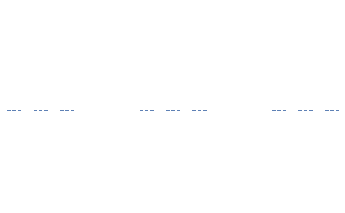
\includegraphics[width=0.3\linewidth]{pics/appendix/1-d_mathematica.png}
        \caption*{The image generated by the above code, here a self-similar set in ambient spatial dimension 1}
    \end{figure}
  
  
  \begin{lstlisting}[language=Mathematica,title={Mathematica code for 2-dimensional images}]
    functions=RandomInteger[{1,3},10000];
    
    f1[j_,x_] := Which[ j ==1, x/2, j==2, x/2, j==3, x/2+1/2 ];
    
    f2[j_,y_] := Which[ j ==1, y/2, j==2, y/2+1/2, j==3, y/2+1/4 ];
    
    sample={{0,0}};
    
    For [ i=1, i<=Length[functions], i++,
    AppendTo[ sample, { f2[functions[[i]],sample[[i]][[1]]],  f1[functions[[i]],sample[[i]][[2]]] }  
    ];
    
    ListPlot[ sample, PlotStyle -> PointSize[0.000000001], AspectRatio -> Automatic, Axes -> {False,False}]
  \end{lstlisting}
  
  \begin{figure}[htb]
        \centering
        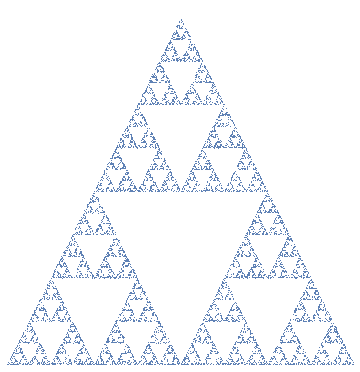
\includegraphics[height=0.5\linewidth]{pics/appendix/2-d_mathematica.png}
        \caption*{The image generated by the above code, here a Sierpi{\'n}ski triangle}
    \end{figure}
  

 
  
  \newpage
  \begin{lstlisting}[language=Mathematica,title={Mathematica code for 3-dimensional images}]
    functions=RandomInteger[{1,4},10000];
    
    f1[j_,x_] :=Which[ j ==1, x/2,
    j==2, x/2,
    j==3, x/2+1/2,
    j==4, x/2+1/4
    ];
    
    f2[j_,y_] := Which[ j ==1, y/2,
    j==2, y/2+1/2,
    j==3, y/2+1/4,            
    j==4, y/2+1/4                   
    ];
    
    f3[j_,z_] := Which[ j ==1, z/2,
    j==2, z/2,
    j==3, z/2 ,                                       
    j==4, z/2+1/2                                                   
    ];
    
    sample={{0,0,0}};
    
    For [ i=1, i<=Length[functions], i++,
    AppendTo[ sample, {
    f1[functions[[i]],sample[[i]][[1]]],  
    f3[functions[[i]],sample[[i]][[2]]],
    f2[functions[[i]],sample[[i]][[3]]]   
    }]
    ];
    
    ListPointPlot3D[ sample, PlotStyle -> PointSize[0.000000001], BoxRatios -> Automatic, Ticks -> None]
  \end{lstlisting}
 
  \begin{figure}[htb]
        \centering
        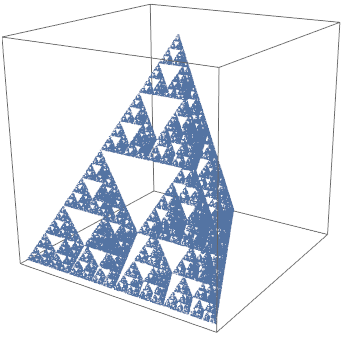
\includegraphics[height=0.5\linewidth]{pics/ch-upper-reg/sierptetra.png}
        \caption*{The image generated by the above code, here a Sierpi{\'n}ski tetrahedron}
  \end{figure}
    
    